\documentclass[10pt, french]{article}
%% -----------------------------
%% Préambule
%% -----------------------------
% !TEX encoding = UTF-8 Unicode
% LaTeX Preamble for all cheatsheets
% Author : Gabriel Crépeault-Cauchon

% HOW-TO : copy-paste this file in the same directory as your .tex file, and add in your preamble the next command right after you have specified your documentclass : 
% \input{preamble-cheatsht.tex}
% ---------------------------------------------
% ---------------------------------------------

% Extra note : this preamble creates document that are meant to be used inside the multicols environment. See the documentation on internet for further information.

%% -----------------------------
%% Encoding packages
%% -----------------------------
\usepackage[utf8]{inputenc}
\usepackage[T1]{fontenc}
\usepackage{babel}
\usepackage{lmodern}

%% -----------------------------
%% Variable definition
%% -----------------------------
\def\auteur{Gabriel Crépeault-Cauchon / Nicholas Langevin}
\def\BackgroundColor{white}

%% -----------------------------
%% Margin and layout
%% -----------------------------
% Determine the margin for cheatsheet
\usepackage[landscape, hmargin=1cm, vmargin=1.7cm]{geometry}
\usepackage{multicol}

% Remove automatic indentation after section/subsection title.
\setlength{\parindent}{0cm}

% Save space in cheatsheet by removing space between align environment and normal text.
\usepackage{etoolbox}
\newcommand{\zerodisplayskips}{%
  \setlength{\abovedisplayskip}{0pt}%
  \setlength{\belowdisplayskip}{0pt}%
  \setlength{\abovedisplayshortskip}{0pt}%
  \setlength{\belowdisplayshortskip}{0pt}}
\appto{\normalsize}{\zerodisplayskips}
\appto{\small}{\zerodisplayskips}
\appto{\footnotesize}{\zerodisplayskips}

%% -----------------------------
%% URL and links
%% -----------------------------
\usepackage{hyperref}
\hypersetup{colorlinks = true, urlcolor = gray!70!white, linkcolor = black}

%% -----------------------------
%% Document policy (uncomment only one)
%% -----------------------------
%	\usepackage{concrete}
	\usepackage{mathpazo}
%	\usepackage{frcursive} %% permet d'écrire en lettres attachées
%	\usepackage{aeguill}
%	\usepackage{mathptmx}
%	\usepackage{fourier} 

%% -----------------------------
%% Math configuration
%% -----------------------------
\usepackage[fleqn]{amsmath}
\usepackage{amsthm,amssymb,latexsym,amsfonts}
\usepackage{empheq}
\usepackage{numprint}
\usepackage{dsfont} % Pour avoir le symbole du domaine Z

% Mathematics shortcuts

\newcommand{\reels}{\mathbb{R}}
\newcommand{\entiers}{\mathbb{Z}}
\newcommand{\naturels}{\mathbb{N}}
\newcommand{\eval}{\biggr \rvert}
\usepackage{cancel}
\newcommand{\derivee}[1]{\frac{\partial}{\partial #1}}
\newcommand{\prob}[1]{\Pr \left( #1 \right)}
\newcommand{\esp}[1]{\mathrm{E} \left[ #1 \right]} % espérance
\newcommand{\variance}[1]{\mathrm{Var} \left( #1   \right)}
\newcommand{\covar}[1]{\mathrm{Cov} \left( #1   \right)}
\newcommand{\laplace}{\mathcal{L}}
\newcommand{\deriv}[2][]{\frac{\partial^{#1}}{\partial #2^{#1}}}
\newcommand{\e}[1]{\mathrm{e}^{#1}}
\newcommand{\te}[1]{\text{exp}\left\{#1\right\}}
\DeclareMathSymbol{\shortminus}{\mathbin}{AMSa}{"39}



% To indicate equation number on a specific line in align environment
\newcommand\numberthis{\addtocounter{equation}{1}\tag{\theequation}}

%
% Actuarial notation packages
%
\usepackage{actuarialsymbol}
\usepackage{actuarialangle}

%
% Matrix notation for math symbols (\bm{•})
%
\usepackage{bm}
% Matrix notation variable (bold style)
\newcommand{\matr}[1]{\mathbf{#1}}



%% -----------------------------
%% tcolorbox configuration
%% -----------------------------
\usepackage[most]{tcolorbox}
\tcbuselibrary{xparse}
\tcbuselibrary{breakable}

%%
%% Coloured box "definition" for definitions
%%
\DeclareTColorBox{definition}{ o }				% #1 parameter
{
	colframe=blue!60!green,colback=blue!5!white, % color of the box
	breakable, 
	pad at break* = 0mm, 						% to split the box
	title = {#1},
	after title = {\large \hfill \faBook},
}
%%
%% Coloured box "definition2" for definitions
%%
\DeclareTColorBox{definitionNOHFILL}{ o }				% #1 parameter
{
	colframe=blue!60!green,colback=blue!5!white, % color of the box
	pad at break* = 0mm, 						% to split the box
	title = {#1},
	before title = {\faBook \quad },
	breakable
}


%%
%% Coloured box "algo" for algorithms
%%
\newtcolorbox{algo}[ 1 ]
{
	colback = blue!5!white,
	colframe = blue!75!black,
	title=#1,
	fonttitle = \bfseries,
	breakable
}
%%
%% Coloured box "conceptgen" for points adding to a concept's deifintion
%%
\newtcolorbox{conceptgen}[ 1 ]
{
	breakable,
	colback = beaublue,
	colframe = airforceblue,
	title=#1,
	fonttitle = \bfseries
}
%%
%% Coloured box "probch3" pour formules relatives au 3ème chapitre de prob
%%
\newtcolorbox{probch3}[ 1 ]
{
	colback = ruddypink,
	colframe = burgundy,
	fonttitle = \bfseries,	
	breakable,
	title=#1
}
%%
%% Coloured box "formula" for formulas
%%
\newtcolorbox{formula}[ 1 ]
{
	colback = green!5!white,
	colframe = green!70!black,
	breakable,
	fonttitle = \bfseries,
	title=#1
}
%%
%% Coloured box "formula" for formulas
%%
\DeclareTColorBox{algo2}{ o }
{
	enhanced,
	title = #1,
	colback=blue!5!white,	
	colbacktitle=blue!75!black,
	fonttitle = \bfseries,
	breakable,
	boxed title style={size=small,colframe=arsenic} ,
	attach boxed title to top center = {yshift=-3mm,yshifttext=-1mm},
}
%%
%% Coloured box "examplebox" for formulas
%%
\newtcolorbox{examplebox}[ 1 ]
{
	colback = lightmauve,
	colframe = antiquefuchsia,
	breakable,
	fonttitle = \bfseries,title=#1
}
%%
%% Coloured box "rappel" pour rappel de formules
%%
\newtcolorbox{rappel}[ 1 ]
{
	colback = ashgrey,
	colframe = arsenic,
	breakable,
	fonttitle = \bfseries,title=#1
}
%%
%% Coloured box "rappel" pour rappel de formules
%%
\DeclareTColorBox{rappel_enhanced}{ o }
{
	enhanced,
	title = #1,
	colback=ashgrey, % color of the box
%	colframe=blue(pigment),
%	colframe=arsenic,	
	colbacktitle=arsenic,
	fonttitle = \bfseries,
	breakable,
	boxed title style={size=small,colframe=arsenic} ,
	attach boxed title to top center = {yshift=-3mm,yshifttext=-1mm},
}
%%
%% Coloured box "notation" for notation and terminology
%%
\DeclareTColorBox{distributions}{ o }			% #1 parameter
{
	enhanced,
	title = #1,
	colback=gray(x11gray), % color of the box
%	colframe=blue(pigment),
	colframe=arsenic,	
	colbacktitle=aurometalsaurus,
	fonttitle = \bfseries,
	boxed title style={size=small,colframe=arsenic} ,
	attach boxed title to top center = {yshift=-3mm,yshifttext=-1mm},
	breakable
%	left=0pt,
%  	right=0pt,
%    box align=center,
%    ams align*
%  	top=-10pt
}

%% -----------------------------
%% Graphics and pictures
%% -----------------------------
\usepackage{graphicx}
\usepackage{pict2e}
\usepackage{tikz}

%% -----------------------------
%% insert pdf pages into document
%% -----------------------------
\usepackage{pdfpages}

%% -----------------------------
%% Color configuration
%% -----------------------------
\usepackage{color, soulutf8, colortbl}


%
%	Colour definitions
%
\definecolor{blue(munsell)}{rgb}{0.0, 0.5, 0.69}
\definecolor{blue(matcha)}{rgb}{0.596, 0.819, 1.00}
\definecolor{blue(munsell)-light}{rgb}{0.5, 0.8, 0.9}
\definecolor{bleudefrance}{rgb}{0.19, 0.55, 0.91}
\definecolor{blizzardblue}{rgb}{0.67, 0.9, 0.93}
\definecolor{bondiblue}{rgb}{0.0, 0.58, 0.71}
\definecolor{blue(pigment)}{rgb}{0.2, 0.2, 0.6}
\definecolor{bluebell}{rgb}{0.64, 0.64, 0.82}
\definecolor{airforceblue}{rgb}{0.36, 0.54, 0.66}
\definecolor{beaublue}{rgb}{0.74, 0.83, 0.9}
\definecolor{cobalt}{rgb}{0.0, 0.28, 0.67}	% nice light blue-ish
\definecolor{blue_rectangle}{RGB}{83, 84, 244}		% ACT-2004
\definecolor{indigo(web)}{rgb}{0.29, 0.0, 0.51}	% purple-ish
\definecolor{antiquefuchsia}{rgb}{0.57, 0.36, 0.51}	%	pastel dark purple ish
\definecolor{darkpastelpurple}{rgb}{0.59, 0.44, 0.84}
\definecolor{gray(x11gray)}{rgb}{0.75, 0.75, 0.75}
\definecolor{aurometalsaurus}{rgb}{0.43, 0.5, 0.5}
\definecolor{ruddypink}{rgb}{0.88, 0.56, 0.59}
\definecolor{pastelred}{rgb}{1.0, 0.41, 0.38}		
\definecolor{lightmauve}{rgb}{0.86, 0.82, 1.0}
\definecolor{azure(colorwheel)}{rgb}{0.0, 0.5, 1.0}
\definecolor{darkgreen}{rgb}{0.0, 0.2, 0.13}			
\definecolor{burntorange}{rgb}{0.8, 0.33, 0.0}		
\definecolor{burntsienna}{rgb}{0.91, 0.45, 0.32}		
\definecolor{ao(english)}{rgb}{0.0, 0.5, 0.0}		% ACT-2003
\definecolor{amber(sae/ece)}{rgb}{1.0, 0.49, 0.0} 	% ACT-2004
\definecolor{green_rectangle}{RGB}{131, 176, 84}		% ACT-2004
\definecolor{red_rectangle}{RGB}{241,112,113}		% ACT-2004
\definecolor{amethyst}{rgb}{0.6, 0.4, 0.8}
\definecolor{amethyst-light}{rgb}{0.6, 0.4, 0.8}
\definecolor{ashgrey}{rgb}{0.7, 0.75, 0.71}			% dark grey-black-ish
\definecolor{arsenic}{rgb}{0.23, 0.27, 0.29}			% light green-beige-ish gray
\definecolor{amaranth}{rgb}{0.9, 0.17, 0.31}
\definecolor{brickred}{rgb}{0.8, 0.25, 0.33}
\definecolor{pastelred}{rgb}{1.0, 0.41, 0.38}

%
% Useful shortcuts for coloured text
%
\newcommand{\orange}{\textcolor{orange}}
\newcommand{\red}{\textcolor{red}}
\newcommand{\cyan}{\textcolor{cyan}}
\newcommand{\blue}{\textcolor{blue}}
\newcommand{\green}{\textcolor{green}}
\newcommand{\purple}{\textcolor{magenta}}
\newcommand{\yellow}{\textcolor{yellow}}

%% -----------------------------
%% Enumerate environment configuration
%% -----------------------------
%
% Custum enumerate & itemize Package
%
\usepackage{enumitem}
%
% French Setup for itemize function
%
\frenchbsetup{StandardItemLabels=true}
%
% Change default label for itemize
%
\renewcommand{\labelitemi}{\faAngleRight}


%% -----------------------------
%% Tabular column type configuration
%% -----------------------------
\newcolumntype{C}{>{$}c<{$}} % math-mode version of "l" column type
\newcolumntype{L}{>{$}l<{$}} % math-mode version of "l" column type
\newcolumntype{R}{>{$}r<{$}} % math-mode version of "l" column type
\newcolumntype{f}{>{\columncolor{green!20!white}}p{1cm}}
\newcolumntype{g}{>{\columncolor{green!40!white}}m{1.2cm}}
\newcolumntype{a}{>{\columncolor{red!20!white}$}p{2cm}<{$}}	% ACT-2005
% configuration to force a line break within a single cell
\usepackage{makecell}


%% -----------------------------
%% Fontawesome for special symbols
%% -----------------------------
\usepackage{fontawesome}

%% -----------------------------
%% Section Font customization
%% -----------------------------
\usepackage{sectsty}
\sectionfont{\color{\SectionColor}}
\subsectionfont{\color{\SubSectionColor}}

%% -----------------------------
%% Footer/Header Customization
%% -----------------------------
\usepackage{lastpage}
\usepackage{fancyhdr}
\pagestyle{fancy}

%
% Header
%
\fancyhead{} 	% Reset
\fancyhead[L]{Aide-mémoire pour~ \cours ~(\textbf{\sigle})}
\fancyhead[R]{\auteur}

%
% Footer
%
\fancyfoot{}		% Reset
\fancyfoot[R]{\thepage ~de~ \pageref{LastPage}}
\fancyfoot[L]{\href{https://github.com/ressources-act/Guide_de_survie_en_actuariat}{\faGithub \ ressources-act/Guide de survie en actuariat}}
%
% Page background color
%
\pagecolor{\BackgroundColor}




%% END OF PREAMBLE
% ---------------------------------------------
% ---------------------------------------------
\usepackage{ulem}
\usepackage{booktabs}
%% -----------------------------
%% Redefine from template
%% -----------------------------
\def\auteur{Alec James van Rassel}
%% -----------------------------
%% Variable definition
%% -----------------------------
\def\cours{Francais}
\def\sigle{alloprof}
%% -----------------------------
%% Colour setup for sections
%% -----------------------------
\def\SectionColor{burntorange}
\def\SubSectionColor{burntsienna}
\def\SubSubSectionColor{burntsienna}
%%%
%%%
%%%
\hypersetup{colorlinks = true, urlcolor = blue, linkcolor = black}
\usepackage{multicol}
\usetikzlibrary{matrix}
\setcounter{secnumdepth}{0}
\setlist{leftmargin=*}
\DeclareTColorBox{astuces}{ o }			% #1 parameter
{
	enhanced,
	title = #1,
	colback=beaublue, % color of the box
%	colframe=blue(pigment),
	colframe=ballblue,	
	colbacktitle=aurometalsaurus,
	fonttitle = \bfseries,
	boxed title style={size=small,colframe=arsenic} ,
	attach boxed title to top center = {yshift=-3mm,yshifttext=-1mm},
%	left=0pt,
%  	right=0pt,
%    box align=center,
%    ams align*
%  	top=-10pt
}

\graphicspath{{src/FRN-3003/}}

%% -----------------------------
%% Début du document
%% -----------------------------
\begin{document}
\raggedcolumns
\begin{multicols*}{2}

\section{La grammaire de la phrase}
\begin{definitionNOHFILL}[Une phrase]
Ensemble syntaxique autonome; c'est-à-dire, les groupes qui composent la phrase forment un énoncé qui se suffit à lui-même.

\begin{definitionNOHFILLsub}[Phrase graphique]
Unité de sens qui commence par une majuscule et qui se termine par un point (d'interrogation, d'exclamation ou trois points de suspension).
\begin{itemize}
	\item	Une même phrase graphique peut contenir plusieurs phrases syntaxiques.
\end{itemize}
\end{definitionNOHFILLsub}%
\begin{definitionNOHFILLsub}[Phrase syntaxique]
Unité de sens qui comprend, au minimum \textbf{le sujet} et \textbf{le prédicat} et possiblement \textbf{le complément de phrase}.
\begin{itemize}
	\item	On peut compter le nombre de phrases syntaxiques dans une phrase graphique en comptant le nombre de verbes conjugés.
\end{itemize}
\end{definitionNOHFILLsub}
\end{definitionNOHFILL}

\subsection{La syntaxe}
%	bon video qui explique la phrase http://monde.ccdmd.qc.ca/ressource/?id=103527
\subsubsection*{Phrase de base}
\begin{center}
\tikzset{every picture/.style={line width=0.75pt}} %set default line width to 0.75pt        

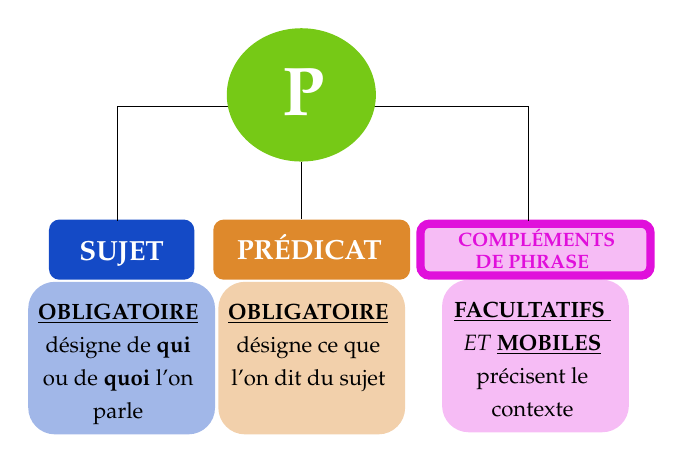
\begin{tikzpicture}[x=0.75pt,y=0.75pt,yscale=-1,xscale=1]
%uncomment if require: \path (0,300); %set diagram left start at 0, and has height of 300

%Flowchart: Alternative Process [id:dp3139800615130719] 
\draw  [draw opacity=0][fill={rgb, 255:red, 20; green, 74; blue, 198 }  ,fill opacity=1 ] (99.83,126.24) .. controls (99.83,123.44) and (102.11,121.17) .. (104.91,121.17) -- (164.76,121.17) .. controls (167.56,121.17) and (169.83,123.44) .. (169.83,126.24) -- (169.83,145.09) .. controls (169.83,147.89) and (167.56,150.17) .. (164.76,150.17) -- (104.91,150.17) .. controls (102.11,150.17) and (99.83,147.89) .. (99.83,145.09) -- cycle ;
%Flowchart: Alternative Process [id:dp5908990075861504] 
\draw  [draw opacity=0][fill={rgb, 255:red, 222; green, 137; blue, 44 }  ,fill opacity=1 ] (179,126.24) .. controls (179,123.44) and (181.27,121.17) .. (184.08,121.17) -- (268.76,121.17) .. controls (271.56,121.17) and (273.83,123.44) .. (273.83,126.24) -- (273.83,145.09) .. controls (273.83,147.89) and (271.56,150.17) .. (268.76,150.17) -- (184.08,150.17) .. controls (181.27,150.17) and (179,147.89) .. (179,145.09) -- cycle ;
%Flowchart: Alternative Process [id:dp05081667220998187] 
\draw  [color={rgb, 255:red, 224; green, 16; blue, 219 }  ,draw opacity=1 ][fill={rgb, 255:red, 224; green, 16; blue, 219 }  ,fill opacity=0.28 ][line width=3]  (278.81,127.54) .. controls (278.81,125.13) and (280.77,123.17) .. (283.18,123.17) -- (385.27,123.17) .. controls (387.68,123.17) and (389.64,125.13) .. (389.64,127.54) -- (389.64,143.79) .. controls (389.64,146.21) and (387.68,148.17) .. (385.27,148.17) -- (283.18,148.17) .. controls (280.77,148.17) and (278.81,146.21) .. (278.81,143.79) -- cycle ;

%Flowchart: Alternative Process [id:dp3172857547525272] 
\draw  [draw opacity=0][fill={rgb, 255:red, 20; green, 74; blue, 198 }  ,fill opacity=0.4 ] (89.83,164.03) .. controls (89.83,156.93) and (95.59,151.17) .. (102.7,151.17) -- (166.97,151.17) .. controls (174.07,151.17) and (179.83,156.93) .. (179.83,164.03) -- (179.83,211.8) .. controls (179.83,218.91) and (174.07,224.67) .. (166.97,224.67) -- (102.7,224.67) .. controls (95.59,224.67) and (89.83,218.91) .. (89.83,211.8) -- cycle ;
%Flowchart: Alternative Process [id:dp49634226268152126] 
\draw  [draw opacity=0][fill={rgb, 255:red, 222; green, 137; blue, 44 }  ,fill opacity=0.4 ] (181.42,164.03) .. controls (181.42,156.93) and (187.18,151.17) .. (194.28,151.17) -- (258.55,151.17) .. controls (265.66,151.17) and (271.42,156.93) .. (271.42,164.03) -- (271.42,211.8) .. controls (271.42,218.91) and (265.66,224.67) .. (258.55,224.67) -- (194.28,224.67) .. controls (187.18,224.67) and (181.42,218.91) .. (181.42,211.8) -- cycle ;
%Flowchart: Alternative Process [id:dp43373109220714334] 
\draw  [draw opacity=0][fill={rgb, 255:red, 224; green, 16; blue, 219 }  ,fill opacity=0.28 ] (289.22,163.03) .. controls (289.22,155.93) and (294.98,150.17) .. (302.09,150.17) -- (366.36,150.17) .. controls (373.47,150.17) and (379.22,155.93) .. (379.22,163.03) -- (379.22,210.8) .. controls (379.22,217.91) and (373.47,223.67) .. (366.36,223.67) -- (302.09,223.67) .. controls (294.98,223.67) and (289.22,217.91) .. (289.22,210.8) -- cycle ;
%Straight Lines [id:da17212294053882182] 
\draw    (132.83,66.67) -- (132.83,121.67) ;
%Straight Lines [id:da5604875139333634] 
\draw    (186.83,66.67) -- (132.83,66.67) ;
%Straight Lines [id:da5581588908691753] 
\draw    (330.83,66.67) -- (330.83,121.67) ;
%Straight Lines [id:da3726917603582094] 
\draw    (330.83,66.67) -- (250.83,66.67) ;
%Straight Lines [id:da838114078832441] 
\draw    (221.42,93.23) -- (221.42,120.73) ;
%Shape: Ellipse [id:dp527152881406457] 
\draw  [draw opacity=0][fill={rgb, 255:red, 118; green, 201; blue, 22 }  ,fill opacity=1 ] (185.5,61.12) .. controls (185.5,43.38) and (201.58,29) .. (221.42,29) .. controls (241.25,29) and (257.33,43.38) .. (257.33,61.12) .. controls (257.33,78.85) and (241.25,93.23) .. (221.42,93.23) .. controls (201.58,93.23) and (185.5,78.85) .. (185.5,61.12) -- cycle ;


% Text Node
\draw (109.83,130.17) node [anchor=north west][inner sep=0.75pt]   [align=left] {\begin{minipage}[lt]{35.600856pt}\setlength\topsep{0pt}
\begin{center}
\textbf{\textcolor[rgb]{1,1,1}{SUJET}}
\end{center}

\end{minipage}};
% Text Node
\draw (187.92,127.17) node [anchor=north west][inner sep=0.75pt]   [align=left] {\begin{minipage}[lt]{54.102500000000006pt}\setlength\topsep{0pt}
\begin{center}
\textbf{\textcolor[rgb]{1,1,1}{PRÉDICAT}}
\end{center}

\end{minipage}};
% Text Node
\draw (295.72,122.37) node [anchor=north west][inner sep=0.75pt]  [font=\scriptsize,color={rgb, 255:red, 224; green, 16; blue, 219 }  ,opacity=1 ] [align=left] {\begin{minipage}[lt]{53.500428pt}\setlength\topsep{0pt}
\begin{center}
\textbf{\textcolor[rgb]{0.88,0.06,0.86}{{\scriptsize COMPLÉMENTS}}}\\{\textbf{\textcolor[rgb]{0.88,0.06,0.86}{{\scriptsize DE PHRASE}}}}
\end{center}

\end{minipage}};
% Text Node
\draw (207.92,47.12) node [anchor=north west][inner sep=0.75pt]   [align=left] {\begin{minipage}[lt]{19.663356pt}\setlength\topsep{0pt}
\begin{center}
\textbf{\textcolor[rgb]{1,1,1}{{\Huge P}}}
\end{center}

\end{minipage}};
% Text Node
\draw (92.83,160.42) node [anchor=north west][inner sep=0.75pt]   [align=left] {\begin{minipage}[lt]{58.63585600000001pt}\setlength\topsep{0pt}
\begin{center}
{\footnotesize \textbf{\underline{OBLIGATOIRE}}}\\{\footnotesize désigne de \textbf{qui}}\\{\footnotesize ou de \textbf{quoi} l'on}\\{\footnotesize parle}
\end{center}

\end{minipage}};
% Text Node
\draw (184.42,160.42) node [anchor=north west][inner sep=0.75pt]   [align=left] {\begin{minipage}[lt]{58.63585600000001pt}\setlength\topsep{0pt}
\begin{center}
{\footnotesize \textbf{\underline{OBLIGATOIRE}}}\\{\footnotesize désigne ce que}\\{\footnotesize l'on dit du sujet}
\end{center}

\end{minipage}};
% Text Node
\draw (292.22,159.42) node [anchor=north west][inner sep=0.75pt]   [align=left] {\begin{minipage}[lt]{58.926216000000004pt}\setlength\topsep{0pt}
\begin{center}
{\footnotesize \textbf{\underline{FACULTATIFS }}}\\{\footnotesize \textit{ET }\textbf{\underline{MOBILES}}}\\{\footnotesize précisent le }\\{\footnotesize contexte }
\end{center}

\end{minipage}};


\end{tikzpicture}
\end{center}
\begin{definitionNOHFILLprop}[cinq aspects]
\begin{enumerate}
	\item	Elle est \textbf{déclarative}.
		\begin{enumerate}
		\item	C.-à-d. qu'elle ne contient aucune marque d'interrogation, d'exclamation et aucune formulation impérative.
		\end{enumerate}
	\item	Elle est \textbf{positive}.
		\begin{enumerate}
		\item	C.-à-d. qu'elle ne comprend aucune marque de négation ;
		\item	Par exemple : les élèves remettent leurs travaux à temps ;
		\item	Comparativement à la forme {\color{teal}négative}: les élèves {\color{teal}ne} remettent {\color{teal}pas} leurs travaux à temps.
		\end{enumerate}
	\item	Elle est \textbf{active}.
		\begin{enumerate}
		\item	C.-à-d. que le groupe nominale ou le pronom sujet est bien celui qui exercice l'action du verbe principal de la phrase et qui est le donneur d'accord.
		\end{enumerate}
	\item	Elle est \textbf{neutre}.
		\begin{enumerate}
		\item	C.-à-d. qu'aucun mot est ajouté pour mettre l'accent sur un élément de la phrase ;
		\item	Par exemple, \og \textbf{C'est} Mélanie \textbf{qui} étudie présentement \fg{}.
		\end{enumerate}
	\item	Elle est \textbf{personnelle}.
		\begin{enumerate}
		\item	C.-à-d. qu'il n'y a pas de formulations impersonnelles ;
		\item	Par exemple, \textit{il y a}, \textit{il faut}, etc.
		\end{enumerate}
\end{enumerate}
\end{definitionNOHFILLprop}

\begin{definitionNOHFILLpropos}[Caractéristiques]
\begin{enumerate}
	\item	Elle commence toujours par une majuscule et se termine par un point.
	\item	Elle est constituée de mots qui forment un ensemble cohérents lorsque réunis dans un ordre précis.
	\item	Elle est composé, au minimum, de : \textbf{\textcolor{teal}{le sujet}} et \textbf{\textcolor{cyan}{le prédicat}}.
		\begin{itemize}
		\item	Le sujet d'abord et le verbe ensuite.
		\end{itemize}
	\item	Elle peut contenir \textbf{le complément de phrase}.
\end{enumerate}
\tcbline
Par exemple, \textcolor{teal}{Chloé} \textcolor{cyan}{parle de sa meilleur amie}.
\end{definitionNOHFILLpropos}


\columnbreak
\subsection{Les marques de ponctuation}
\begin{definitionNOHFILL}[Le point (.)]
Termine généralement une phrase déclarative ou impérative.\\

\begin{itemize}
	\item	Généralement, on ne mets pas de point dans un titre.
\end{itemize}
\end{definitionNOHFILL}

\begin{astuces}[Énumération verticale]
Chaque item est complété d'un point-virgule sauf le dernier qui a un point.\\

Par exemple :
\begin{itemize}
	\item	des oreilles \textbf{;}
	\item	des mains \textbf{;}
	\item	une tête\textbf{.}
\end{itemize}
\end{astuces}

\begin{definitionNOHFILLprop}[Le point d'exclamation (!)]
Exprime l'exclamation.

Soit le point d'exclamation : 
\begin{enumerate}
	\item	Marque la fin d'une phrase exclamative ;
	\item	Termine une phrase exclamative non verbale ;
	\item	Marque la fin d'une interjection.
		\begin{itemize}
		\item	Dans ce cas-ci il peut ou pas être suivi d'une majuscule.
		\end{itemize}
\end{enumerate}
\end{definitionNOHFILLprop}

\begin{definitionNOHFILLprop}[Le point d'interrogation (?)]
Marque une interrogation.

\begin{astuces}[Phrase interrogative suivie d'une incise]
Si la phrase interrogative est suivie d'une incise, l'incise ne commencera pas par une lettre majuscule.	\\

Par exemple: C'est votre sœur qui l'a tué ? \textit{d}emanda-t-il poliment.
\end{astuces}
\end{definitionNOHFILLprop}

\begin{definitionNOHFILLprop}[Les point de suspension (...)]
Signe de ayant de différentes utilités : 
\begin{enumerate}
	\item	Marquer la fin d'une phrase ; 
		\begin{itemize}
		\item	Marque la fin d'une phrase, la prochaine lettre est une majuscule.
		\end{itemize}
	\item	Marque la continuité d'une abréviation ;
		\begin{itemize}
		\item	Indique qu'une énumération est volontairement écourtée ;
		\item	La prochaine lettre est une majuscule.
		\end{itemize}
	\item	Marque l'hésitation dans un discours ; 
		\begin{itemize}
		\item	Marque une hésitation de l'auteur ;
		\item	La prochaine lettre sera une \textbf{minuscule} ;
		\item	Son rôle devient équivalent à celui du point-virgule.
		\end{itemize}
	\item	Marque l'absence d'un passage dans une citation ;
		\begin{itemize}
		\item	On indique un passage coupé par \textbf{[...]}.
		\end{itemize}
	\item	Autres fonctions.
		\begin{itemize}
		\item	
		\end{itemize}
\end{enumerate}
\end{definitionNOHFILLprop}

\begin{definitionNOHFILLprop}[Le point abréviatif]
Indique que la fin d'un mot a été supprimée.	\\

Par exemple :
\begin{itemize}
	\item	282 pages -> 282 p.
\end{itemize}

\begin{astuces}[Abréviations sans point abréviatif]
On ne met pas de point abréviatif aux abréviations se terminant par la dernière lettre du mot, les symboles, les sigles et les acronymes.	\\

Par exemple : 
\begin{itemize}
	\item	numéro -> no.
	\item	kilogramme -> kg
	\item	Organisation des Nations Unies -> ONU
\end{itemize}
\end{astuces}
\end{definitionNOHFILLprop}

\begin{definitionNOHFILL}[La virgule]

\end{definitionNOHFILL}

\begin{definitionNOHFILLprop}[Le point-virgule]

\end{definitionNOHFILLprop}

\begin{definitionNOHFILLprop}[Les deux points]

\end{definitionNOHFILLprop}

\subsubsection{Accolades et. al.}

\begin{definitionNOHFILLprop}[Les parenthèses]

\end{definitionNOHFILLprop}

\begin{definitionNOHFILLprop}[Les guillemets]

\end{definitionNOHFILLprop}

\begin{definitionNOHFILLprop}[Les crochets]

\end{definitionNOHFILLprop}

\begin{definitionNOHFILLprop}[Le tiret]

\end{definitionNOHFILLprop}

\begin{definitionNOHFILLprop}[La barre oblique]

\end{definitionNOHFILLprop}

\subsubsection{Autres}

\begin{definitionNOHFILLprop}[Les marques du paragraphe]

\end{definitionNOHFILLprop}




\newpage
\section{Classes de mots}
\subsection{Le nom}
\begin{definitionNOHFILL}[Le nom]
Mot qui désigne une "réalité" ; c'est-à-dire, une personne, un animal, un objet, un lieu, un événement, une époque, un concept abstrait, etc.	\\

Généralement, le nom : 
\begin{enumerate}
	\item	a un genre qui lui est propre (masculin ou féminin) ;
	\item	peut varier en nombre (singulier ou pluriel) ;
	\item	est précédé d'un déterminant.
\end{enumerate}
\end{definitionNOHFILL}

\subsubsection*{Types de noms}
%	https://www.francaisfacile.com/exercices/exercice-francais-2/exercice-francais-84631.php
\begin{definitionNOHFILLsub}[Le nom commun]
Mot qui s'écrit avec une lettre \textbf{minuscule} et qui désigne des individus de la même espèce ; il correspond à un concept.

\begin{itemize}
	\item	Il est généralement accompagné d'un déterminant.
\end{itemize}

\tcbline

Exemples :
\begin{itemize}
	\item	un être : personne, gars, fille, etc.
	\item	une chose : voiture, ballon, brosse, etc.
	\item	une notion : peur, amour, destin, etc.
\end{itemize}
\end{definitionNOHFILLsub}
\begin{definitionNOHFILLsub}[Le nom propre]
Mot qui s'écrit avec une lettre \textbf{majuscule} et qui s'applique à une chose (ou une collection de choses, un lieu, une personne) unique qu'il désigne.

\begin{itemize}
	\item	Il n'est pas généralement accompagné d'un déterminant ;
	\item	Il faut distinguer les noms propres des adjectifs de nationalité qui sont écrits en minuscules.
\end{itemize}

\tcbline

Exemples :
\begin{itemize}
	\item	un être : \textbf{G}eorge, \textbf{L}inda, \textbf{A}lec, etc.
	\item	une notion : l'\textbf{H}omme, l'\textbf{A}mour, \textbf{D}ieu, etc.
	\item	un lieu : \textbf{F}rance, \textbf{Q}uébec, les montages \textbf{R}ocheuses, etc.
	\item	une période historique : \textbf{M}oyen \textbf{Â}ge, \textbf{R}enaissance, etc.
	\item	une divinité : \textbf{Z}eus, \textbf{M}ercure, etc.
	\item	un point cardinal : la Rive-\textbf{S}ud, le \textbf{N}ord canadien, etc.
	\item	une fête : \textbf{N}oël, \textbf{H}alloween, etc.
	\item	un peuple : les \textbf{Q}uébécois, les \textbf{C}anadiens, etc.
\end{itemize}
\end{definitionNOHFILLsub}


\subsubsection*{Caractéristiques des noms}
\begin{definitionNOHFILLpropos}[Caractère animé ou inanimé]
Exemples si le nom désigne :
\begin{itemize}
	\item	quelque chose animé (de vivant) : lion, éléphant, athlète, etc.
		\begin{itemize}
		\item	Généralement, les noms qui désignent des êtres animés varient en genre ;
		\item	Par exemple, la lionne et le lion.
		\end{itemize}
	\item	des objets inanimés : ordinateur, crayon, voiture, etc.
		\begin{itemize}
		\item	Généralement, les noms qui désignent des objets inanimés ne varient pas en genre ;
		\item	Par exemple, la nuit, le livre, etc.
		\end{itemize}
\end{itemize}
\end{definitionNOHFILLpropos}


\begin{definitionNOHFILLpropos}[Trait humain ou non humain]
Les noms qui désignent une réalité
\begin{itemize}
	\item	\textbf{propre à} l'espèce humaine a un \textbf{\textit{trait humain}}
		\begin{itemize}
		\item	Par exemple : visage, notaire, Diane, ongles, bouche, etc.
		\end{itemize}
	\item	qui \textbf{n'appartient pas} à l'espèce humaine a un \textbf{\textit{trait non humain}}
		\begin{itemize}
		\item	Par exemple : canard, bec, griffe, gueule, etc.
		\end{itemize}
\end{itemize}
\begin{astuces}[Astuce]
Le trait humain ou non humain fait partie des caractéristiques à observer dans le choix du pronom relatif.
\end{astuces}
\end{definitionNOHFILLpropos}


\begin{definitionNOHFILLpropos}[Trait comptable ou non comptable]
Les noms avec le trait : 
\begin{description}
	\item[comptable]	peuvent être accompagnés d'un déterminant numéral.
		\begin{itemize}
		\item	Par exemple : huit chandails, cent individus, etc.
		\end{itemize}
	\item[non comptable]	sont accompagnés de déterminants partitifs.
		\begin{itemize}
		\item	Par exemple : du poivre, du courage, de l'huile, etc.
		\end{itemize}
\end{description}

\begin{astuces}[Astuce]
Certains noms peuvent avoir le trait comptable dans une situation, mais pas dans une autre.\\
Le truc est soit de vérifier si le nom est quantifiable ou le déterminant qui convient le mieux à la situation.

\tcbline

Exemple :
\begin{itemize}
	\item	Je vois \textbf{trois} chevaux. (trait comptable)
	\item	Je mange \textbf{du} cheval. (trait non comptable)
\end{itemize}
\end{astuces}
\end{definitionNOHFILLpropos}

\begin{definitionNOHFILLpropos}[Trait individuel ou collectif]
\begin{itemize}
	\item	Exemples de mots qui désignent une réalité distincte : chat, individu, garçon, etc.
	\item	Exemples de mots qui désignent une réalité collective : peuple, troupeau, groupe, etc.
\end{itemize}
\end{definitionNOHFILLpropos}

\begin{definitionNOHFILLpropos}[Trait concret ou abstrait]
Les noms qui :
\begin{itemize}
	\item	ont un caractère concret représentent des réalités perceptible par les sens ont un trait  concret.
		\begin{itemize}
		\item	Par exemple : chien, eau, télévision, vent, etc.
		\end{itemize}
	\item	représentent des idées ou des réalités que l'on ne perçoit pas par les sens ont un trait abstrait.
		\begin{itemize}
		\item	Par exemple : idée, hypothèse, haine, violence, confiance, etc.
		\end{itemize}
\end{itemize}
\end{definitionNOHFILLpropos}


\subsubsection*{Genre et nombre}
Tel que mentionné, les noms qui varient en genre ont un caractère animé.
\begin{astuces}[Exceptions du pluriel de noms finissant en \textit{ou}]
Tout les noms qui finissent en \textit{ou} ont un \textit{s} ajouté pour le pluriel excepté :
\begin{multicols*}{2}
\begin{description}
	\item[bijou\textbf{x}]
	\item[caillou\textbf{x}]
	\item[chou\textbf{x}]
	\item[genou\textbf{x}]
	\item[hibou\textbf{x}]
	\item[joujou\textbf{x}]
	\item[pou\textbf{x}]
\end{description}
\end{multicols*}
\end{astuces}

\begin{astuces}[Exceptions du pluriel de mots finissant en \textit{ail}]
Tout les noms qui finissent en \textit{ail} ont un \textit{s} ajouté pour le pluriel excepté :
\begin{multicols*}{2}
\begin{description}
	\item[bail/b\textbf{aux}]
	\item[corail/cor\textbf{aux}]
	\item[émail/ém\textbf{aux}]
	\item[soupirail/soupir\textbf{aux}]
	\item[travail/trav\textbf{aux}]
	\item[vantail/vant\textbf{aux}]
	\item[vitrail/vitr\textbf{aux}]
\end{description}
\end{multicols*}
\end{astuces}

\subsubsection*{Majuscule ou minuscule ?}
Questions à se poser.
Est-ce un :
\begin{enumerate}
	\item	nom propre ou un adjectif ?
		\begin{itemize}
		\item	Les \textbf{F}rançais vs du vin \textbf{f}rançais.
		\item	Les noms propres indiquant les nationalités ont des majuscules alors que les adjectifs de nationalité ont des minuscules.
		\end{itemize}
	\item	nom propre ou nom commun ?
		\begin{itemize}
		\item	Par exemple, les : mois (\textbf{j}anvier), langues (le \textbf{n}orvégien), religions (le \textbf{b}uddhisme), jours (\textbf{l}undi), fonctions ou titres civils (le \textbf{p}remier ministre)
		\end{itemize}
\end{enumerate}

Le nom désigne-t-il :
\begin{enumerate}
	\setcounter{enumi}{2}
	\item	un emplacement géographique ?
		\begin{itemize}
		\item	Les noms de lieux prennent (généralement) des lettres majuscules, mais le le nom commun le précédent s'écrit avec une minuscule ;
		\item	Par exemple : \textbf{Asie}, \textbf{P}aris, l'océan \textbf{P}acifique, la montagne \textbf{N}oire.
		\end{itemize}
	\item	un astre ?
		\begin{itemize}
		\item	Les noms de constellations, d'étoiles et de planètes prennent une majuscule ;
		\item	L'adjectif qui l'accompagne prend une majuscule uniquement s'il le précède ;
		\item	Par exemple : la \textbf{L}une, la planète \textbf{M}ars, la \textbf{G}rande \textbf{O}urse, la \textbf{V}oie \textbf{l}actée, etc.
		\end{itemize}
	\item	une période ou un fait historique ?
		\begin{itemize}
		\item	Les noms qui désignent une période ou un fait historique prennent une majuscule ;
		\item	L'adjectif qui l'accompagne prend une majuscule uniquement s'il le précède ;
		\item	Par exemple : l'\textbf{Antiquité}, le \textbf{M}oyen \textbf{Â}ge, la \textbf{R}évolution française, la \textbf{G}rande \textbf{D}épression.
		\end{itemize}
	\item	un point cardinal ?
		\begin{itemize}
		\item	Sauf si ils sont employés adjectivement ou qu'ils représentent une direction ou orientation, ils sont écrits avec une lettre majuscule ;
		\item	Par exemple : le pôle \textbf{N}ord, l'Amérique du \textbf{S}ud, la rue Sainte-Catherine \textbf{E}st, \og ensuite tu roules vers le \textbf{n}ord \fg{}, l'hémisphère \textbf{s}ud, \og la maison est à l'\textbf{o}uest de la ville \fg{}.
		\end{itemize}
	\item	une fête religieuse (ou nationale) ?
		\begin{itemize}
		\item	Le nom qui désigne spécifiquement la fête prend une majuscule ;
		\item	Par exemple : la fête du \textbf{T}ravail, le jour du \textbf{S}ouvenir, le jour de l'\textbf{A}n, le \textbf{M}ardi gras, etc.
		\end{itemize}
	\item	un ministère ?
		\begin{itemize}
		\item	Le nom qui désigne spécifiquement le ministre dont il s'agit prend une majuscule, le mot \textit{ministère} comme tel n'en prend jamais ;
		\item	Par exemple : le ministère de la \textbf{J}ustice, le ministère des \textbf{A}ffaires culturelles, 
		\end{itemize}
\end{enumerate}

Le groupe de mots désigne-t-il :
\begin{enumerate}
	\setcounter{enumi}{8}
	\item	une organisation ?
		\begin{itemize}
		\item	\textbf{Seul le premier mot} prend une majuscule ;
		\item	Par exemple : l'\textbf{É}cole nationale de l'humour, la \textbf{F}aculté des sciences et de génie, le \textbf{C}ercle des fermieres de \textbf{T}rois-\textbf{R}ivières, etc.
		\end{itemize}
\end{enumerate}


\columnbreak
\subsection{Le déterminant}
\begin{definitionNOHFILL}[Le déterminant]
Mot qui sert à introduire un mot dans la phrase.\\

\begin{itemize}
	\item	Précède un nom.
	\item	Receveur d'accord; reçoit le genre et nombre du nom qu'il accompagne.
\end{itemize}
\end{definitionNOHFILL}


\subsubsection{L'article}
\textbf{L'article}
\begin{center}
\begin{tabular}{| >{\columncolor{airforceblue}}c | >{\columncolor{beaublue}}c  |}
\hline
défini	&	le, la, les	\\\hline
indéfini	&	un, une, des	\\\hline
partitif	&	du, de, la, de l'\\\hline
\end{tabular}
\end{center}

\begin{definitionNOHFILLsub}[Article défini]
Désignent précisément une chose (personne, espèce ou une réalité connue).		\\

Exemples : 
\begin{itemize}
	\item	Elle a rencontrée \textbf{l}'homme de sa vie.
	\item	J'adore \textbf{la} musique.
	\item	\textbf{Les} enfants à Sharon ont grandis !
\end{itemize}
\end{definitionNOHFILLsub}

\begin{definitionNOHFILLsub}[Article indéfini]
Désignent une chose (personne, etc.) mais pas de façon précise.	\\

Exemples : 
\begin{itemize}
	\item	J'ai vu \textbf{un} singe au zoo.
	\item	Marco a \textbf{une} faim de loup.
	\item	Ils possèdent \textbf{des} voitures élégantes.
\end{itemize}
\end{definitionNOHFILLsub}

\begin{definitionNOHFILLsub}[Article partitif]
Désignent une quantité de matière (réelle ou non).	\\

\begin{itemize}
	\item	Employé devant un nom que l'on ne peut pas compter (eau, sable, farine, etc.).
\end{itemize}

\

Exemples : 
\begin{itemize}
	\item	Les abeilles fabriquent \textbf{du} miel.
	\item	Je vais acheter \textbf{du} lait et \textbf{du} fromage.
	\item	Peux-tu me donner \textbf{de} l'eau stp ?
\end{itemize}
\end{definitionNOHFILLsub}

\begin{astuces}[Article vs pronom]
Devant un verbe, le, la, les ou l' sont des \textbf{\textit{pronoms}}.
\begin{itemize}
	\item	Il mange \textbf{la} pomme. (article)
	\item	Il \textbf{la} trouve excellente ! (pronom qui remplacement le nom pomme)
\end{itemize}
\end{astuces}

\begin{astuces}[Article indéfini vs article défini contractée \textit{des}]
Si l'on peut remplacer \lfbox[conditions]{\textbf{des}} par l'article défini \lfbox[conditions]{\textbf{les}}, c'est un article indéfini sinon c'est un article défini contractée.
\end{astuces}

\begin{astuces}[Article partitif vs article défini contracté \textit{du}]
Si l'on peut remplacer \lfbox[conditions]{\textbf{du}} par \lfbox[conditions]{\textbf{un peu de}}, c'est un article partitif.
\end{astuces}


\subsubsection{Les déterminants}
\begin{definitionNOHFILLsub}[Déterminant démonstratif]
Désignent plus particulièrement une personne (un objet).\\

Soit :
\begin{itemize}
	\item	Ce, cet(te) ou ces.
\end{itemize}

\

Exemples :
\begin{itemize}
	\item	\textbf{Cette} \textit{maison} est centenaire.
	\item	\textbf{Ces} \textit{enfants} jouent au ballon à tous les jours.
\end{itemize}
\end{definitionNOHFILLsub}
\begin{astuces}[Déterminant démonstratif renforcé par un adverbe]
On peut aussi ajouter les adverbes \textit{ci} et \textit{là} après le nom pour renforcer le déterminant démonstratif. \textit{Ci} indique une idée de proximité alors que \textit{là} exprime une idée d'éloignement.	\\

Exemples : 
\begin{itemize}
	\item	\textbf{Cette} \textit{fille}-\textbf{là} est tellement gentille ! 
	\item	Je dois passer \textbf{ce} \textit{cours}-\textbf{ci} cet automne.
\end{itemize}
\end{astuces}

\begin{definitionNOHFILLsub}[Déterminant possessif]
Désignent une possession, une relation d'appartenance, de paternité, d'origine, etc.\\

Exemples :
\begin{itemize}
	\item	\textbf{Sa} maison.
	\item	\textbf{Ton} automobile.
	\item	\textbf{Leurs} responsabilités.
\end{itemize}
\end{definitionNOHFILLsub}

\begin{definitionNOHFILLsub}[Déterminant interrogatif]
Employés dans les interrogations directes et indirectes.\\

Soit :
\begin{itemize}
	\item	\textbf{quel[s](le[s])}, ou
	\item	les déterminants invariables \textbf{combien d'} et \textbf{que d'}.
\end{itemize}

\

Exemples :
\begin{itemize}
	\item	Je me demande \textbf{quelle} \textit{famille} oserait vivre ici.
	\item	Je lui ai demandé \textbf{quel} est son \textit{age}.
\end{itemize}
\end{definitionNOHFILLsub}

\begin{definitionNOHFILLsub}[Déterminant exclamatif]
Employés dans phrases exclamatives.	\\

Soit :
\begin{itemize}
	\item	\textbf{quel[s](le[s])}, ou
	\item	les déterminants invariables \textbf{combien d'} et \textbf{que d'}.
\end{itemize}

\

Exemples :
\begin{itemize}
	\item	\textbf{Quel} beau \textit{paysage} ! 
	\item	\textbf{Quelle} \textit{fille} extraordinaire ! 
	\item	\textbf{Que de} \textit{bêtises} ils ont commises ! 
\end{itemize}
\end{definitionNOHFILLsub}

\begin{definitionNOHFILLsub}[Déterminant numéral]
Désignent un nombre et sont suivis d'un nom.	\\

Exemples :
\begin{itemize}
	\item	zéro, quarante-deux, etc.
\end{itemize}
\end{definitionNOHFILLsub}

\begin{definitionNOHFILLsub}[Déterminant quantitatif]
Introduisent un nom en donnant une indication sur sa quantité.	\\

Exemples :
\begin{itemize}
	\item	\textbf{N'importe quelle} voiture.
	\item	\textbf{Quelques} livres.
	\item	\textbf{Aucun} élève.
\end{itemize}
\end{definitionNOHFILLsub}

\begin{definitionNOHFILLsub}[Déterminant relatif]
Sert à introduire un nom déjà utilisé ou suggéré dans une phrase. Il est plutôt rare et surtout utilisé dans les textes officiels.

Soit : 
\begin{itemize}
	\item	Lequel / lesquels et laquelle / lesquelles.
	\item	Duquel / desquels et de laquelle / desquelles.
	\item	Auquel / auxquels et à laquelle / auxquelles.
\end{itemize}

\

Exemples : 
\begin{itemize}
	\item	Je vais vous donner un ordinateur, lequel ordinateur sera très performant.
	\item	La mère de James, laquelle mère a été prévenue de comparaître, sera au tribunal pour répondre à des questions importantes.
\end{itemize}
\end{definitionNOHFILLsub}


\columnbreak
\subsection{Les adjectifs}
\begin{definitionNOHFILLsub}[Adjectifs de nationalité]
%	https://www.francaisfacile.com/exercices/exercice-francais-2/exercice-francais-118858.php
Majuscule ou minuscule ?
\begin{itemize}
	\item	Nom d'une lange $\Rightarrow$ minuscule
		\begin{itemize}
		\item	Par exemple, Vous parlez \textbf{e}spagnol.
		\end{itemize}
	\item	Adjectif qualifiant un nom $\Rightarrow$ minuscule
		\begin{itemize}
		\item	Par exemple, Un artiste \textbf{a}nglais m'a vendu cette peinture.
		\end{itemize}
	\item	Nom désignant un habitant $\Rightarrow$ majuscule
		\begin{itemize}
		\item	Par exemple, Un \textbf{A}nglais m'a parlé hier.
		\end{itemize}
\end{itemize}
\end{definitionNOHFILLsub}


\columnbreak
\subsection{Le pronom}
\begin{definitionNOHFILL}[Le pronom]
Mot qui sert notamment à la \textbf{reprise d'information} puisqu'il remplace généralement un mot (ou groupe de mots) précédemment nommé.

\begin{itemize}
	\item	P. ex., personne, lieu, objet, etc.
	\item	Ce  type de pronom est un \textbf{pronom de reprise}.
	\item	Le pronom varie en genre et en nombre selon l'antécédent.
\end{itemize}
\end{definitionNOHFILL}

P. ex., si l'antécédent est un groupe :
\begin{description}
	\item[nominal]	\textit{Julien} est parti. \textbf{Il} ne reviendra pas.
	\item[adjectival]	Émilie est \textit{jolie}. Ses sœurs \textbf{le} sont aussi.
	\item[adverbial]	Est-ce que Julie sera \textit{là} ? Elle \textbf{y} sera, comptez là-dessus ! 
	\item[prépositionnel]	Faites-vous partie \textit{de ce groupe} ? Oui, j'\textbf{en} fais partie.
	\item[verbal infinitif]	J'ai voulu \textit{remplacer ce cadre}, mais je ne \textbf{l}'ai pas fait.
	\item[une phrase complète]	\textit{J'ai patiné, j'ai lancé et j'ai compté} ! \textbf{Ceci} en moins de 10 secondes
\end{description}

\begin{definitionNOHFILLsub}[Pronom nominal]
Pronom dont le sens ne provient pas d'un antécédent; le pronom peut posséder une signification propre ou s'expliquer par la situation de communication.

\tcbline

Exemples :
\begin{itemize}
	\item	\textbf{Quelqu'un} a refermé la porte.
	\item	\textbf{Personne} ne l'a vu venir !
	\item	\textbf{Rien} n'explique son comportement.
	\item	Je ne veux plus voir \textbf{ça} dans ta chambre. (\textit{pronom de communication})
\end{itemize}
\end{definitionNOHFILLsub}

\begin{definitionNOHFILLsub}[Pronom personnel]
Mot qui indique la personne grammaticale et peut être un pronom de reprise ou nominal.

\tcbline

P. ex., si le pronom personnel a la fonction du :
\begin{description}
	\item[sujet]	je, tu, il, elle, on, etc. 
	\item[complément]	me, moi, toi, nous, le, elle, soi 
\end{description}
\end{definitionNOHFILLsub}

\begin{definitionNOHFILLsub}[Pronom possessif]
Mot qui remplace une personne (objet, animal) en indiquant qui est le possesseur ou en établissant une relation d'appartenance entre le pronom et son \textit{antécédent}.

\tcbline

Exemples :
\begin{itemize}
	\item	le mien, le tien, la nôtre, la leur, les siens.
\end{itemize}

\textbf{Exemple de phrase} : J'ai trouvé \textit{les cahiers} de tout le monde ! \textbf{Le tien} et \textbf{le mien} sont dans l'armoire.
\end{definitionNOHFILLsub}

\begin{definitionNOHFILLsub}[Pronom démonstratif]
Remplace une personne (objet, animal) que l'on désire montrer.

\tcbline

Exemples :
\begin{itemize}
	\item	celui, celui-ci, celui-là ;
	\item	celle, celle-ci, celle-là ;
	\item	ce, ceci, cela, ça.
\end{itemize}

\textbf{Exemple de phrase} : J'ai pris deux crayons. \textbf{Celui-ci} est bleu, \textbf{celui-là} est jaune.
\end{definitionNOHFILLsub}

\begin{definitionNOHFILLsub}[Pronom relatif]
Mot qui remplace un nom (un "antécédent") et qui introduit une \textit{subordonnée relative}.

\tcbline

Le choix de pronom relatif dépend de sa fonction dans la phrase subordonnée.
\begin{astuces}[Trouver la fonction du pronom relatif]
On disjoint la phrase principale (\textbf{P1}) et la phrase subordonnée (\textbf{P2}) en deux phrases autonomes :
\begin{itemize}
	\item	Le gâteau \textcolor{teal}{\textbf{que} j'ai mangé} était délicieux.
		\begin{description}
		\item[P1]	Le gâteau était délicieux.
		\item[P2]	J'ai mangé \textbf{le gâteau}.
		\end{description}
\end{itemize}

Pour trouver la fonction du pronom relatif \textbf{que} dans la \textcolor{teal}{phrase subordonnée}, il faut trouver la fonction du groupe répétée dans la \textbf{P2} (\textit{\textbf{le gâteau}}).\\
Dans ce cas-ci, \textbf{que} occupe la fonction du \underline{complément direct} comme le groupe nominal \textit{\textbf{le gâteau}} dans \textbf{P2}.
\end{astuces}

Si le pronom occupe la fonction :
\begin{itemize}
	\item	du \textbf{sujet} de la \textbf{P2}.
		\begin{itemize}
		\item	P. ex. : lequel, laquelle, lesquels, qui, etc.
		\end{itemize}
	\item	Complément direct du verbe ou l'attribut du sujet.
		\begin{itemize}
		\item	P. ex. : que (qu')
		\end{itemize}
	\item	Complément de phrase indiquant le lieu ou le temps.
		\begin{itemize}
		\item	P. ex. : où
		\end{itemize}
	\item	Complément indirect du verbe, complément de l'adjectif ou le complément du nom.
		\begin{itemize}
		\item	P. ex. : dont
		\end{itemize}
\end{itemize}
\end{definitionNOHFILLsub}

\begin{astuces}[Conjonction vs pronom \textbf{que}]
Léa m'a dit \textbf{que} tu étais passé.
\begin{itemize}
	\item	Dans ce cas, \textbf{que} est une conjonction qui n'a pas pour fonction de remplacer et n'a pas d'antécédent.
\end{itemize}

La lettre que j'ai écrite est postée.
\begin{itemize}
	\item	Dans ce cas, \textbf{que} est un pronom qui remplace le nom \textit{lettre}.
\end{itemize}
\end{astuces}

\begin{definitionNOHFILLsub}[Pronom interrogatif]
Remplace une personne (objet, animal) ou un élément abstrait sur lequel on se questionne.
\begin{itemize}
	\item	Peut être directe ou indirecte.
\end{itemize}

\tcbline

Exemples:
\begin{itemize}
	\item	\textbf{Que} fabrique-t-elle\textbf{?} (\textit{directe})
	\item	Je me demande \textbf{ce qu}'elle fabrique. (\textit{indirecte})
\end{itemize}
\begin{center}
	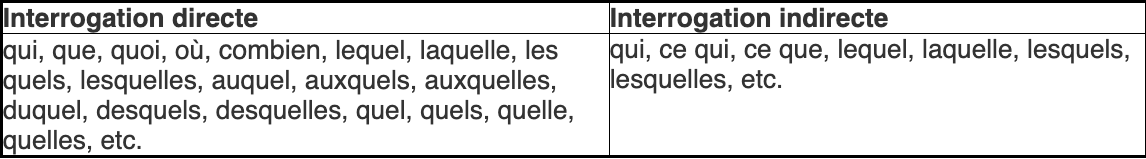
\includegraphics[width=0.9\columnwidth]{pronom-interg}
\end{center}
\end{definitionNOHFILLsub}

\begin{definitionNOHFILLsub}[Pronom indéfini]
Mot qui remplace une personne (objet, animal) d'une manière indéterminée, imprécise.

\tcbline

\begin{itemize}
	\item	Souvent des pronoms nominaux (sans antécédents) mais peut aussi s'agir de pronoms de reprise.
		\begin{itemize}
		\item	\textbf{Chacun} poursuit un rêve, mais \textbf{tous} n'arriveront pas à le réaliser. (pronoms nominaux)
		\item	Quand \textit{les jeunes filles} arrivèrent, je constatai qu'\textbf{aucune} n'avait le matériel nécessaire. (pronom de reprise)
		\end{itemize}
\end{itemize}

\begin{center}
	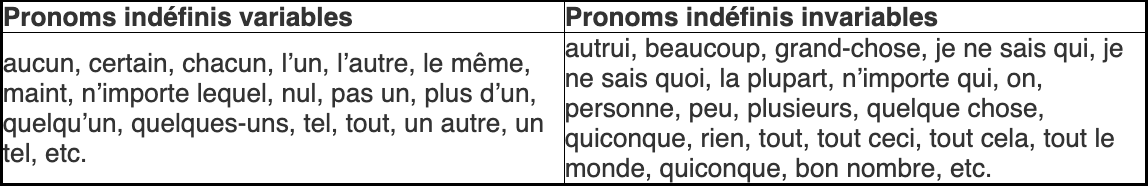
\includegraphics[width=0.9\columnwidth]{pronom-indef}
\end{center}
\end{definitionNOHFILLsub}

\begin{definitionNOHFILLsub}[Pronom numéral]
Pronom de reprise qui précise une quantité.

\tcbline

Par exemple: deux, vingt, trois, etc.
\end{definitionNOHFILLsub}

\begin{astuces}[Pronoms vs déterminants \textbf{numéraux}]
La différence est que le pronom numéral n'accompagne pas un nom.
\end{astuces}


\columnbreak
\subsection{Le verbe}


\columnbreak
\subsection{L'adverbe}
\begin{definitionNOHFILLsub}[Adverbe]
Mot invariable qui modifie ou précise le sens d'un verbe ou adjectif.
\begin{itemize}
	\item	Il peut être effacé de la phrase ;
	\item	Alias, une locution adverbiale.
\end{itemize}

\tcbline

Exemples:
\begin{itemize}
	\item	ainsi, hier, complètement, ici (\textit{adverbes simples}) ;
	\item	en effet, peu à peu, en dessous, c'est-à-dire (\textit{adverbes complexes}) ;
\end{itemize}
\begin{astuces}[Comment repérer un adverbe]
Trouver les mots invariables d'une phrase, ceux qui peuvent être retirés sont des mots invariables.\\
Exemple:	Il semble \textbf{\color{teal}vraiment} concerné \textbf{par} cet avis. On voit que \textbf{\color{teal}vraiment} est l'adverbe.
\end{astuces}
\end{definitionNOHFILLsub}


\subsection{La préposition}
\begin{definitionNOHFILL}[La préposition]
Mot invariable qui unit des mots en les mettant en rapport et qui complète et précise le message présent dans la phrase.
\begin{itemize}
	\item	C'est un mot de liaison;
	\item	Il crée un lien de dépendance entre des éléments syntaxiques.
\end{itemize}

\tcbline

Par exemple:	sur, chez, de, pour, etc.
\end{definitionNOHFILL}

\subsubsection*{Types de prépositions}
\begin{definitionNOHFILLsub}[Prépositions simples]
Prépositions qui ne sont pas décomposables.
\begin{center}
	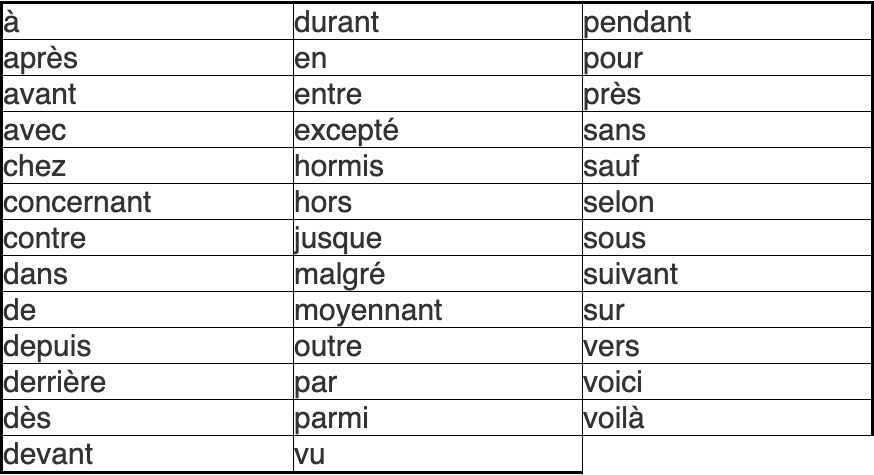
\includegraphics[width=0.9\columnwidth]{prep-simple}
\end{center}
\begin{astuces}[On n'ajoute pas la préposition \textit{de} devant d'autres.]
\paragraph{Exemple :}	Il avait besoin \textit{\sout{de} d'autres} pommes.
\end{astuces}
\end{definitionNOHFILLsub}

\begin{definitionNOHFILLsub}[Prépositions complexes]
Prépositions qui sont décomposables.
\begin{itemize}
	\item	Alias, des locutions prépositives.
\end{itemize}
\begin{center}
	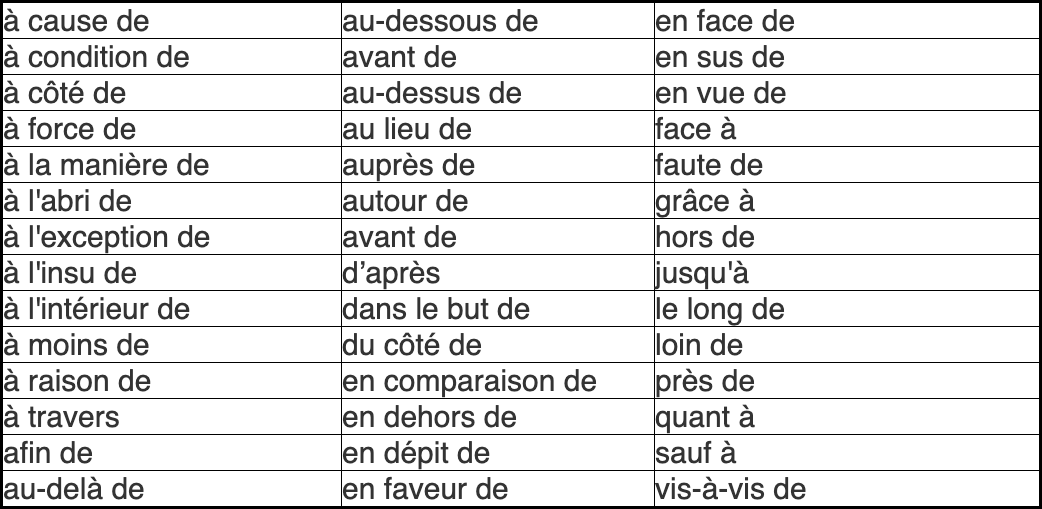
\includegraphics[width=0.9\columnwidth]{prep-compl}
\end{center}
\end{definitionNOHFILLsub}

\begin{definitionNOHFILLsub}[Prépositions contractées]
Prépositions qui ne sont pas décomposables.
\begin{itemize}
	\item	Alias, les déterminants contractés.
\end{itemize}
\begin{center}
	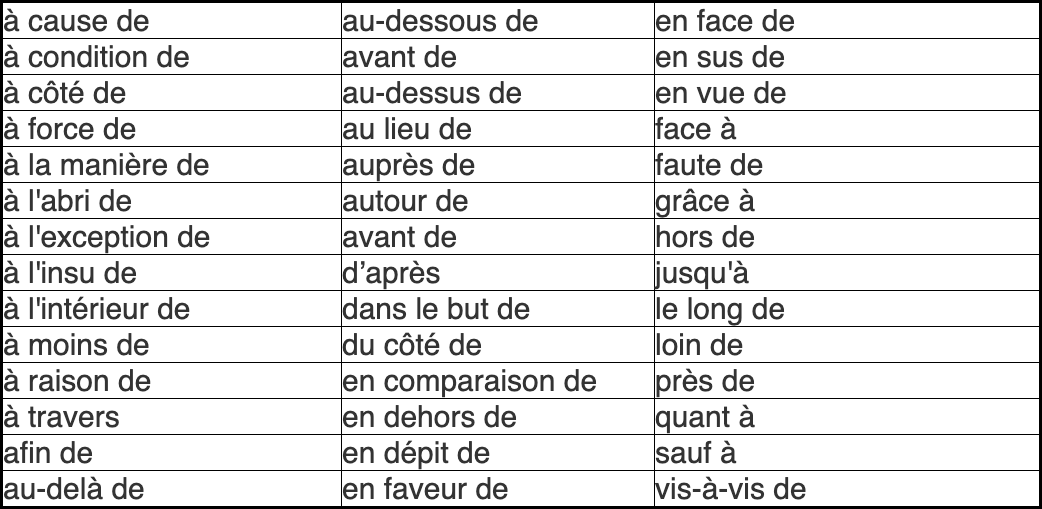
\includegraphics[width=0.9\columnwidth]{prep-compl}
\end{center}

\end{definitionNOHFILLsub}


\columnbreak
\subsection{La conjonction}


\columnbreak
\subsection{L'interjection}
\begin{definitionNOHFILL}[Interjection]
Mot (ou groupe de mots) qui traduit l'émotion de l'énonciateur, sa réaction ou un ordre.
\begin{definitionNOHFILL}[Onomatopées]
Mots classés dans les interjections qui imitent des bruits réels.
\end{definitionNOHFILL}
\begin{itemize}
	\item	L'interjection est suivie d'un point d'exclamation ;
	\item	Si une interjection est composée de plusieurs mots, c'est une \textit{locution interjective}.
\end{itemize}
\tcbline

Exemples:
\begin{itemize}
	\item	Haut les mains ! Mon Dieu ! Ma foi ! (\textit{locutions interjectives}) ;
	\item	Flûte ! Fantastique ! Tiens ! (\textit{nom}, \textit{adjectif}, \textit{verbe}) ;
	\item	Boom ! Ouf ! Aïe ! (\textit{onomatopées}).
\end{itemize}
\end{definitionNOHFILL}


\columnbreak
\subsection{La locution}
\begin{definitionNOHFILL}[La locution]
%	http://www.alloprof.qc.ca/BV/pages/f1233.aspx
Groupe de mots qui forme une unité lexicale. \\
C'est-à-dire: 
\begin{enumerate}[label = \roman*)]
	\item	un adverbe, 
	\item	un verbe,
	\item	une préposition,
	\item	une conjonction ou une interjection composée d'au moins deux mots.
\end{enumerate}

\tcbline

\begin{definitionNOHFILLsub}[Locution adverbiale]
Construite à partir d'un adverbe :
\begin{center}
\begin{tabular}{| >{\columncolor{beaublue}}c | >{\columncolor{beaublue}}c  |}
\hline\rowcolor{airforceblue} 
\textcolor{white}{\textbf{Construction}}	&	\textcolor{white}{\textbf{Exemples}}		\\\specialrule{0.1em}{0em}{0em} 
adverbe + \textbf{adverbe}	&	là-bas, bientôt	\\\hline
préposition + \textbf{adverbe}	&	à jamais, d'ailleurs	\\\hline
\end{tabular}
\end{center}
\end{definitionNOHFILLsub}

\begin{definitionNOHFILLsub}[Locution verbale]
Construite à partir d'un verbe :
\begin{center}
\begin{tabular}{| >{\columncolor{beaublue}}c | >{\columncolor{beaublue}}c  |}
\hline\rowcolor{airforceblue} 
\textcolor{white}{\textbf{Construction}}	&	\textcolor{white}{\textbf{Exemples}}		\\\specialrule{0.1em}{0em}{0em} 
\textbf{verbe} + (déterminant) + nom	&	avoir l'air, rendre l'âme,avoir lieu	\\\hline
\end{tabular}
\end{center}
\end{definitionNOHFILLsub}

\begin{definitionNOHFILLsub}[Locution prépositive]
Construite à partir d'une préposition :
\begin{center}
\begin{tabular}{| >{\columncolor{beaublue}}m{5cm} | >{\columncolor{beaublue}}c  |}
\hline\rowcolor{airforceblue} 
\textcolor{white}{\textbf{Construction}}	&	\textcolor{white}{\textbf{Exemples}}		\\\specialrule{0.1em}{0em}{0em} 
\textbf{préposition} + \textbf{préposition} (ou adverbe)	&	autour de, par-dessus	\\\hline
\textbf{préposition} + (déterminant) + nom + \textbf{préposition}	&	à l'égard de, par rapport à	\\\hline
nom + \textbf{préposition}	&	face à, grâce à	\\\hline
adverbe + \textbf{préposition}	&	contrairement à	\\\hline
\end{tabular}
\end{center}
\end{definitionNOHFILLsub}

\begin{definitionNOHFILLsub}[Locution conjonctive]
Construite à partir d'une conjonction :
\begin{center}
\begin{tabular}{| >{\columncolor{beaublue}}c | >{\columncolor{beaublue}}c  |}
\hline\rowcolor{airforceblue} 
\textcolor{white}{\textbf{Construction}}	&	\textcolor{white}{\textbf{Exemples}}		\\\specialrule{0.1em}{0em}{0em} 
préposition + \textbf{que}	&	avant que, pour que	\\\hline
adverbe + \textbf{que}	&	aussitôt que, bien que	\\\hline
préposition + nom + \textbf{que}	&	à condition que, de crainte que	\\\hline
\end{tabular}
\end{center}
\end{definitionNOHFILLsub}
\end{definitionNOHFILL}

\begin{definitionNOHFILL}[Mot invariable]
Mots qui s’écrivent généralement toujours de la même manière et dont la forme ne dépend pas d'un autre mot.

\tcbline

Par exemple:	la préposition, l'adverbe, etc.
\end{definitionNOHFILL}


\newpage
\section*{\href{http://www.alloprof.qc.ca/bv/pages/f1128.aspx}{La phrase}}

\subsection*{\href{http://www.alloprof.qc.ca/BV/Pages/f1130.aspx}{Le sujet}}
\begin{description}
	\item[Description technique]	Le sujet est une \textbf{fonction} grammaticale qui régit l'accord du verbe;
	\item[Description moins technique]	C'est le \og groupe \fg{} qui donne au verbe son nom et sa personne;
		\begin{itemize}[leftmargin = *]
		\item	On dit \og groupe \fg{} car la fonction sujet est souvent occupée par un \href{http://www.alloprof.qc.ca/BV/pages/f1235.aspx}{groupe du nom};
		\item	Par exemple \og le petit Louis \fg{}, \og les hommes \fg{}, \og les voitures \fg{}.
		\end{itemize}
	\item[Sur le plan sémantique]	il indique \textbf{de qui} ou \textbf{de quoi} on parle dans la phrase.
\end{description}

\begin{distributions}[La fonction sujet peut être occupée par:]
\begin{description}
%%%	--------------------
%%%	NOTE
%%%	+	De quoi qui me manque en compréhension ici pour GN (AJVR).
%%%	--------------------
	\item[Le groupe nominal]	\textbf{GNs};
	\item[Le pronom]	on dit \textbf{pronom sujet};
		\begin{itemize}[leftmargin = *]
		\item	\textcolor{blue_rectangle}{Elles} veulent se rappeler de ce moment tout leur vie.
		\item	\textcolor{blue_rectangle}{Nous} désirons vous rencontrer dans les plus brefs délais.
		\item	\textcolor{blue_rectangle}{Je} suis confortable dans ce lit.
		\end{itemize}
	\item[Le groupe du verbe à infinitif]	on dit \textbf{groupe infinitif sujet};
		\begin{itemize}[leftmargin = *]
		\item	\textcolor{blue_rectangle}{Manger trois repas par jour} est une habitude de vie saine.
		\item	\textcolor{blue_rectangle}{Se marier} est le rêve de bien des gens.
		\item	\textcolor{blue_rectangle}{Étudier} est la clé à la réussite.
		\item	Les groupes on donc un verbe à l'infinitif comme noyau.
		\end{itemize}
	\item[La subordonnée complétive]	on dit \textbf{subordonnée complétive sujet}
		\begin{itemize}[leftmargin = *]
		\item	\textcolor{blue_rectangle}{Qu'il pleuve} change le programme de ma journée.
		\item	\textcolor{blue_rectangle}{Que tu m'appelles} me comble de joie.
		\item	\textcolor{blue_rectangle}{Que tu sois récompensé} est bien normal.
		\item	Les groupes comportent donc un subordonnant \textit{(qu', que)} et un verbe conjugué \textit{(pleuve, appelles, sois récompensé)}.
		\end{itemize}
\end{description}
\end{distributions}

\begin{astuces}[Trucs pour trouver le sujet dans une phrase]
\begin{enumerate}[leftmargin = *]
	\item	Poser la question \textit{Qu'est-ce qui ?} ou \textit{Qui est-ce qui ?} devant le verbe.
	\item	Encadrer le sujet par \textbf{C'est \dots qui} ou \textbf{Ce sont \dots qui}.
	\item	Remplacer le sujet par un pronom (procédé appelé la \textbf{pronominalisation}).
		\begin{itemize}[leftmargin = *]
		\item	Par exemple, remplacer \og Alec aime apprendre \fg{} par \og il aime apprendre \fg{}.
		\end{itemize}
\end{enumerate}
\end{astuces}

\paragraph{NOTE}	Le sujet de la phrase est \textbf{non-effaçable} sinon elle n'a plus de sens. On  dit donc que le sujet est un \textbf{constituant obligatoire} de la phrase.


\subsection*{\href{http://www.alloprof.qc.ca/BV/Pages/f1131.aspx}{Le prédicat}}

\subsection*{\href{http://www.alloprof.qc.ca/BV/Pages/f1132.aspx}{Le complément de phrase}}



%\begin{tikzpicture}
%\clip node (m) [
%	matrix,
%	matrix of nodes,
%	fill = black!20, % alternating rows color
%	inner sep = 1pt, % width of exterior line
%	nodes in empty cells,
%	nodes = {
%		minimum height = 1cm,
%		minimum width = 2.6cm,
%		anchor = center,
%		outer sep = 0,
%		font = \sffamily
%	},
%	row 1/.style = {
%		nodes = {
%			fill = ballblue,  % header colour
%			text = white,
%			font = \bfseries
%		}
%	},
%%	column 1/.style = {
%%		nodes = {
%%			fill = gray,
%%			text = white,
%%			align = right,
%%			text width = 2.5cm,
%%			text depth = 0.5ex
%%		}
%%	},
%	column 1/.style = {
%		text width = 4cm, 
%		align = center,
%		nodes = {
%			font = \bfseries
%		},
%		every even row/.style = {
%			nodes = {
%				fill = white
%			}
%		}
%	},
%	column 2/.style = {
%		text width = 3cm,
%		align = center,
%		every even row/.style = {nodes = {fill = white}},
%	},
%%	row 1 column 1/.style = {nodes = {fill = gray}},
%	prefix after command = {
%		[rounded corners = 4mm] (m.north east) rectangle (m.south west)
%	}
%] {
%	Norwegian	&	English \\
%	Jeg	&	I	\\
%	du	&	you	\\
%	han	&	he	\\
%	hun	&	she	\\
%	det	&	it	\\
%};
%\end{tikzpicture}
%
%\subsection*{Verbs}
%\begin{tikzpicture}
%\clip node (m) [
%	matrix,
%	matrix of nodes,
%	fill = black!20, % alternating rows color
%	inner sep = 1pt, % width of exterior line
%	nodes in empty cells,
%	nodes = {
%		minimum height = 1cm,
%		minimum width = 2.6cm,
%		anchor = center,
%		outer sep = 0,
%		font = \sffamily
%	},
%	row 1/.style = {
%		nodes = {
%			fill = ballblue,  % header colour
%			text = white,
%			font = \bfseries
%		}
%	},
%%	column 1/.style = {
%%		nodes = {
%%			fill = gray,
%%			text = white,
%%			align = right,
%%			text width = 2.5cm,
%%			text depth = 0.5ex
%%		}
%%	},
%	column 1/.style = {
%		text width = 4cm, 
%		align = center,
%		nodes = {
%			font = \bfseries,
%			fill = lightgray
%		}
%	},
%	column 2/.style = {
%		text width = 3cm,
%		align = center,
%		nodes = {
%			fill = white
%		}
%	},
%	column 3/.style = {
%		text width = 3cm,
%		align = center,
%		nodes = {
%			font = \bfseries,
%			fill = lightgray
%		}
%	},
%	column 4/.style = {
%		text width = 3cm,
%		align = center,
%		nodes = {
%			fill = white
%		}
%	},
%%	row 1 column 1/.style = {nodes = {fill = gray}},
%	prefix after command = {
%		[rounded corners = 4mm] (m.north east) rectangle (m.south west)
%	}
%] {
%	Singular	&	&	Plural	&\\
%	Jeg er	&	I am	&	vi er	&	we are	\\
%	du er	&	you are	&	dere er	&	 you are	\\
%	han, hun, det, er	&	he, she, it, is	&	de er	&	they are	\\
%};
%\end{tikzpicture}

\end{multicols*}
%% -----------------------------
%% Fin du document
%% -----------------------------
\end{document}
